\documentclass[12pt,a4paper]{report}

\usepackage[dutch]{babel}
\usepackage{colortbl}

\usepackage{caption}
\captionsetup[figure]{slc=off} % "slc" is an abbreviation for "singlelinecheck"

\usepackage{geometry}
\geometry{a4paper,total={180mm,257mm},left=20mm,top=20mm}

\usepackage{graphicx}
\DeclareGraphicsExtensions{.pdf,.png,.jpg}

\begin{document}

\title{
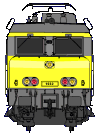
\includegraphics[scale=2.0]{images/rcu_logo}
\makebox[\linewidth]{\rule{\textwidth}{0.4pt}}
Railclub Utrecht
\vfill
Uitbreiding centrale H0 groep\\
\makebox[\linewidth]{\rule{\textwidth}{0.4pt}}
\vfill
\small
\author{Peter Mansvelder}}

\maketitle

\begin{figure}[ht]
  \captionbox
  {Terugmeldschakeling centrale}
  {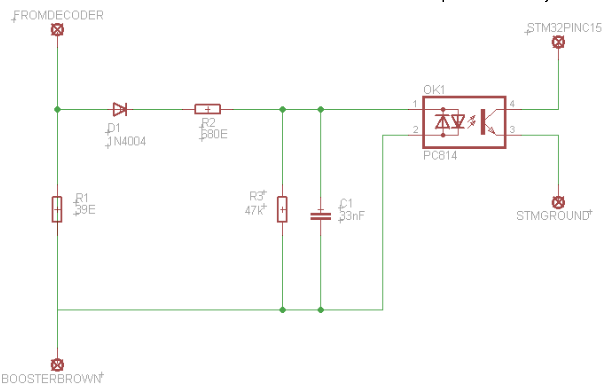
\includegraphics[scale=0.7]{images/rcu-MDRRCII-ack}}
\end{figure}

\begin{itemize}
\item Weerstand 39 Ohm
\item Weerstand 680 Ohm
\item Weerstand 47kOhm
\item Diode 1N4004
\item Optocoupler PC814
\item Condensator 33nF
\end{itemize}

\end{document}
